\section{Algorithm}

In this section we describe the components of our algorithm and their
relationship with each other.  The algorithm predicts the syntactic
category of a word in a given context based on its substitutes.  In
other words first we construct the co-occurrence representation of
words and their substitutes with the help of a language model and then
map each value in the co-occurrence data to a corresponding embedding
on a $n$ dimensional sphere using the S-CODE algorithm.  Finally, we
apply k-means clustering to categorize the word embeddings by which we
induced the word categories.  In the next subsection we detail the
construction of co-occurrence representation of the input, in
Subsection~\ref{sec:cooc} we explain the embedding calculation and
finally in Subsection~\ref{??} we describe the different ways of
embedding clustering.\todo{do we need subsections?}

\subsection{Co-occurences}
\label{sec:cooc}
% How we represent the context?
% How we relate the word and the context?

Word contexts are represented by substitutes sampled from the
corresponding substitute word distributions.  Substitute words are
sampled with replacement from the substitute distributions that are
calculated based on an n-gram language model.  The calculation of
substitute distributions and substitute sampling are detailed in
Appendix~\ref{sec:subcomp}.\todo{appendix section requires edit} The
sample space of the substitute word distributions is the vocabulary of
the language model.\footnote{Sampled substitutes might include the
  unknown word tag ``unk'' since it is in the language model
  vocabulary.  For example substitutes of proper nouns usually include
  ``\_unk\_'' as a substitute.}  To capture the relation between each
word and its context we construct a co-occurrence representation by
pairing the words with their sampled substitutes.
Table~\ref{tab:samples} shows sampled substitutes of each word and
their co-occurrence representation on an example sentence.  A word
might appear as a target word or a sampled substitute therefore to
clarify this ambiguity we concatenate ``W'' and ``S'' to words and
substitutes, respectively, on the co-occurrence data.

The next section explains the S-CODE algorithm which takes the
co-occurrence data as its input and calculates the embeddings of the
words and their substitutes on an $n$ dimensional sphere.  In the rest
of paper we use the term ``substitutes'' to refer ``sampled
substitutes''.

\begin{table}[h]
\caption{The left table shows three possible substitutes, seperated
  with ``/'', sampled for each of the positions in the example
  sentence \textit{``Pierre Vinken, 61 years old, will join the board
    as a nonexecutive director Nov.~29 .''} based on a 4-gram language
  model.  The right table represents the input sentence as a
  co-occurrences of words and their substitutes.  Thus words on the
  left column represents the target word while words on the right
  column represents the context of the correponding target word.}
\begin{tabular}{|ll|} \hline
\textbf{Word} & \textbf{Sampled Substitutes}\\
\hline
Pierre & \textit{Mr.}  / \textit{Pierre} /  \textit{Mr.}\\
Vinken & \textit{\_unk\_} / \textit{Beregovoy} / \textit{Cardin}\\
, & \textit{,} / \textit{,} / \textit{,}\\
61 & \textit{48} / \textit{52} / \textit{41}\\
years & \textit{years} /  \textit{years} /  \textit{years}\\
old & \textit{old} /  \textit{old} /  \textit{old}\\
, & \textit{,} /  \textit{,} /  \textit{,}\\
will & \textit{will} /  \textit{will} /  \textit{will}\\
join & \textit{head} /  \textit{join} /  \textit{leave}\\
the  & \textit{its} /  \textit{its} /  \textit{the}\\
board & \textit{board} /  \textit{company} / \textit{firm}\\
as & \textit{as} / \textit{as} / \textit{as}\\
a & \textit{a} / \textit{a} / \textit{a}\\
nonexecutive & \textit{nonexecutive} / \textit{non-executive} / \textit{nonexecutive}\\
director & \textit{chairman} / \textit{chairman} / \textit{director}\\
Nov. & \textit{April} / \textit{May} / \textit{of}\\
29 & \textit{16} /  \textit{29} / \textit{9}\\
. & \textit{.}  / \textit{.} / \textit{.}\\
\hline
\end{tabular}
\quad
\begin{tabular}{|ll|}
\hline
\textbf{Word} & \textbf{Substitute}\\
\hline
W:Pierre & \textit{S:Mr.}\\
W:Pierre & \textit{S:Pierre}\\
W:Pierre & \textit{S:Mr.}\\
W:Vinken & \textit{S:unk}\\
W:Vinken & \textit{S:Beregovoy}\\
W:Vinken & \textit{S:Cardin}\\
\hdots&\\
W:join & \textit{S:head}\\
W:join & \textit{S:join}\\
W:join & \textit{S:leave}\\
W:the & \textit{S:its}\\
W:the & \textit{S:its}\\
W:the & \textit{S:the}\\
\hdots&\\
W:director & \textit{S:chairman}\\
W:director & \textit{S:chairman}\\
W:director & \textit{S:director}\\
\hdots&\\
\hline
\end{tabular}
\label{tab:samples}
\end{table}

\subsection{Co-occurence Embedding}

The S-CODE algotirhm maps each word and substitute value in the
co-occurence data to an embedding on an $n$ dimensional sphere as
detailed in Appendix~\ref{sec:codethr}.  The basic idea of the mapping
is that words and substitutes that are frequently observed as pairs in
the co-occurence data will have close embeddings while unobserved
pairs will have embeddings that are apart from each other.
Table~\ref{fig:scodeexample} illustrates the final output of the
S-CODE for the given example co-occurence data.

\begin{table}[ht]
  \begin{minipage}[t]{.3\textwidth}
    \small
    \begin{tabular}{|l|l|}
        \hline
        \textbf{Word} & \textbf{Substite} \\
        \hline
        \hdots&\\
        W:director & S:chairman \\
        W:chief & S:chairman \\
        \hdots&\\
        W:Pierre & S:Mr. \\
        W:Frank & S:Mr. \\
        \hdots&\\
        \hline
    \end{tabular}
  \end{minipage}
  \begin{minipage}[t]{.7\textwidth}
    \centering
    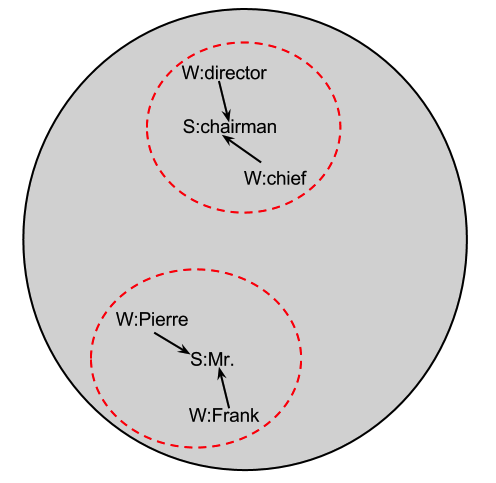
\includegraphics[height=.70\textwidth]{scode-ex.png}\\
    \vspace{-10 mm}
  \end{minipage}
  \caption{The table on the left is a sample co-occurence data that is
    input to the S-CODE algorithm.  The figure on the right is the
    embeddings on the sphere after S-CODE converges.  Dashed circles
    represent the possible groupings of the embeddings on the sphere.}
  \label{fig:scodeexample}
\end{table}

The sample co-occurence data in Table~\ref{fig:scodeexample} consists
of pairs such as (\textit{W:director}, \textit{S:chairman}) and
(\textit{W:chief}, \textit{S:chairman}) therefore S-CODE forces the
embeddings of \textit{W:director} and \textit{W:chief} to be close to
the embeddings of \textit{S:chairman}.  As a results on the output of
S-CODE the embeddings of \textit{W:director} and \textit{W:chief} will
be close to each other due to the shared subsitute
\textit{S:chairman}.


\subsection{Co-occurence Embedding Clustering}


